\section{Design and Implementation}
% General
% Describe how you have chosen to solve the problem
% Argue clearly for the choices made when designing and developing the solution.
LSH is an efficient and space efficient algorithm which makes it ideal to perform a nearest neighbour search. Combined with other techniques this has been used as the bases for the detection of plagiarised documents.

% Explain that special characters have been removed, e.g hash value of "explain," != "explain"


\paragraph{Wikiparser}
% Binary search to find location of article in index file.
% Decision to unzip small amount and process at a time.
The \emph{Wikipedia} database is provided as a compressed archive of articles in the open-source \emph{bzip2} format with an accompanied index file listing the contents of the archive. Because the articles are formatted in XML and wikitext\footnote{A special markup language used by Wikipedia to format plain text into articles} the space of the compressed archive is significantly reduced. Because of the sheer amount of data, decompressing and keeping every article in memory is simply infeasible. We have circumvented this issue by performing an on-the-fly, as-needed decompression of articles while they are fed to the LSH algorithm. This reduces the necessary amount of memory to only keeping a block (100 articles) in memory at a time. This operation is performed by reading the index file line by line, in which the start and end position of the data block can be found, then seeking and reading that block in the compressed archive file, decompressing and parsing the XML structure to separate articles. The implementation is achieved by overriding the \texttt{\_\_iter\_\_} and \texttt{\_\_next\_\_} methods from the \emph{Python} programming language to create an iterable object.

Another much needed functionality is fast lookup of articles. This is desirable because we quickly want to retrieve articles which has been marked as plagiarised. Because we have no intend the decompress the article archive (and waste hard drive space) we want to perform the decompression on-the-fly. Since the index file is ordered by the article id we can perform binary search and find the requested article in $\log(u)$ time. Although this binary search is mostly trivial, we have to take special care when seeking in the file since the position of file pointer is not guaranteed to be placed at the start of a new line. Following the binary search we can decompress the block and parse the XML as before.

\paragraph{LSH}
%Normally will the LSH algorithm hash the words of the shingles of a document $k$ times with a different seed value combining the hash values of each shingle with an XOR\footnote{\url{https://en.wikipedia.org/wiki/XOR_gate}} operation to a single hash value, to create $k$ different hash values, that will be the signature of a document. This means that each word in every shingle is hashed $k$ times. A way to improve this, which is implemented in the solution, is by hashing the words in each shingle once, thereby generating one hash value for each shingle. This hash value is then hashed $k$ times with a different seed to generate $k$ different hash values.

% Argue for the choice of parameters like q, r, b, k....
The LSH algorithm has a few different parameters, that should be set according to what you wish to achieve. One of them is the size of the shingles, $q$. For the matching of whole documents $q = 9$, as it is considered safe for large documents.\cite{leskovec2014mining}. % Write something about the value of q for matching paragraphs
The remaining two parameters are $b$ and $r$, which is the number of bands and the number of rows in each band respectively. Chosing these parameters, will change the probability of the signatures in our datastructure of becoming a candidate. With $b=20$ and $r=5$ we get the following curve as seen in figure~\ref{fig:lsh}. This gives us that when the similarity of two documents are $0.51$, then the probability of becoming a candidate is $>1/2$.

\begin{figure}[h]
	\centering
    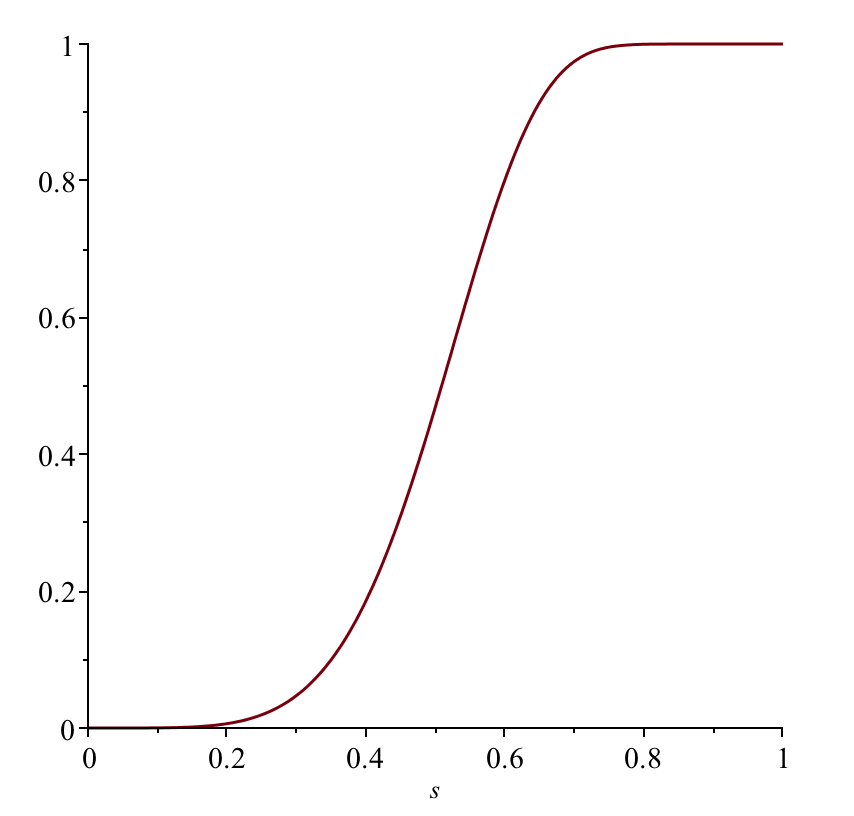
\includegraphics[width = 0.4\linewidth]{docs/report/input/lsh.png}
    \captionsetup{width = \linewidth}
    \caption{Probability of becoming a candidate versus Jaccard similarity of documents of choices of $b=20$ and $r=5$, $1-(1-s^r)^b$}
    \label{fig:lsh}
\end{figure}

\paragraph{Database}
% Show design of tables
% Argue why a database was used
Although LSH is a space efficient datastructure and algorithm there is a trade-off between space and accuracy. Hashing many documents will inevitably grow beyond the amount what can be stored in memory. Storing the LSH datastructure on disk will incur a performance penalty but will enable the datastructure to grow in order of magnitudes larger than what we can fit in memory. We have chosen a database management system (specifically \emph{SQLite}) to store the LSH datastructure. This is a nice abstraction because we can rely on the database for performance and optimisation of the queries. The design of the database schemes can be seen in table~\ref{table:sqlite1} and~\ref{table:sqlite2} and is comprised of two tables (\emph{hashes} and \emph{documents}) in which the attribute \emph{id} is a foreign key referencing the \emph{hashes} table. This allows the database to only store the LSH band once and associate multiple documents to that band.

To assist with lookup performance both tables have indices on critical attributes. The \emph{hashes} table has a combined index on the \emph{hash, band} attributes while the \emph{documents} table has an index on the the \emph{id} attribute alone. This is useful because a usual operation is the check, whether and band is already stored in the database (so as to only store it once). Both tables has a set of constraints such that no two identical bands can be stored and no article can be added to the same band twice (since this information is redundant).

\begin{table}[ht]
    \begin{minipage}[b]{0.56\linewidth}
        \centering
        \begin{tabular}{|l|l|l|}
            \hline
            id (int) & hash (bytes{[}4{]}) & band (int) \\ \hline
            0        & 0xa3f723e8          & 1          \\ \hline
            1        & 0x21be6122          & 1          \\ \hline
            2        & 0xc945e851          & 2          \\ \hline
        \end{tabular}
        \caption{Table \emph{hashes} which stores information on each LSH band with the hash value and the band id}
        \label{table:sqlite1}
    \end{minipage}\hfill
    \begin{minipage}[b]{0.4\linewidth}
        \centering
        \begin{tabular}{|l|l|}
            \hline
            id (int) & doc\_id (int) \\ \hline
            0        & 22            \\ \hline
            1        & 29            \\ \hline
            2        & 22            \\ \hline
        \end{tabular}
        \caption{Table \emph{documents} which associates documents with LSH bands from table \emph{hashes}}
        \label{table:sqlite2}
    \end{minipage}
\end{table}

\paragraph{MapReduce} TODO


% Describe the design and implementation of the solution to find similar documents
% Describe how the original solution was extended to find similar paragraphs